\title{Report on \\ Model Development for Fossil Fuel Divestment}
\author{Jakob J. Kolb \\ Potsdam Institute for Climate Impact Research}

\maketitle

\section{Model Development}

Previous studies \cite{Ans2013} suggest that feedback through supply-demand price mechanisms will have only limited impact on fossil fuel companies. This is due to the fact, that only approximately 15 \% of investors invest subject to socially responsible guidelines \cite{SIF2014Report} and that divested holdings are, especially in liquid markets, very likely to quickly find their way to less responsible investors. \\
Therefore, the effects of a divestment campaigns on target industries rather stem from `soft' factors such as changes in market norms and stigmatization and growing uncertainty about future business opportunities. This means that for the understanding of the campaign dynamics, opinion spreading with respect to beliefs about future business development and respective uncertainties amongst investors might be worth a closer look. \\
In the following I propose a preliminary scheme of such a model.

\begin{figure}[h]
	\centering
	\includegraphics[width = .7 \textwidth]{figures/Model_Scheme.pdf}
	\caption{Schematic sketch of the model including four major components: Households, Firms (grouped by sector), Ecosystem and optional Policy makers.}
	\label{fig:model}
\end{figure}

\subsection{Ramsey-Cass-Koopmans Model of optimal saving}


\subsection{Sectors}

Production is assumed to take place in two sectors. One sector $(d)$ employs a dirty technology depending on fossil resources, the other sector $(c)$ employs a clean technology relying on renewable resources. The physical capital is assumed to be bound to this technology, e.g. there are two separate capital stocks $K_d$ and $K_c$. Both sectors use capital $K_j$ and labor $P_j$ as input factors, the dirty sector additionally uses a fossil resource $R$.
\begin{equation}
	Y_j = F_j(K_j,P_j,R), \qquad \frac{\partial Y_c}{\partial R} = 0 	
	\label{eq:production}
\end{equation}
For the inputs of labor $P$ and capital $K_j$, a Cobb-Douglas type production function is assumed. For the fossil resource input, a Leontief type production function is assumed, since energy (coming from the fossil resource) can only poorly be substituted in general. This results in the following production functions:
\begin{align}
	Y_c &= b_c K_c^{\kappa_c} P_c^{\pi_c} \\
	Y_d &= {\rm min}(b_d K_d^{\kappa_d} P_d ^{\pi_d}, e R)
\end{align}
where $e$ is the fossil resource efficiency.
The total cost for fossil resource extraction $c_R$ (exploration and exploitation) is assumed to scale with $R^{\varepsilon}$.
\begin{equation}
	c_R = b_R R_d^{\varepsilon}
	\label{resource_extraction_cost}
\end{equation}
The factor $b_R$ is presumably depending on the remaining Fossil resource $G$ and increasing as the remaining resource decreases. It is assumed to diverge, as $G$ approaches zero. Also, efficient allocation of resource is assumed, e.g. there are no idle resources in the dirty sector. Consequently, :
\begin{equation}
	Y_d = b_d K_d^{\kappa_d} P_d^{\pi_d} = e R
	\label{efficient_resource_extraction}
\end{equation}
We assume perfect labor mobility, resulting in equal wages in both sectors. We also assume that on the labor and capital market, sectors are price takers, meaning, that wages and capital rental rates are equal to the marginal increase in output per unit input. (Note that in the dirty sector, increase in input factors also result in increasing resource costs $c_R$):
For wages, this results in the following conditions:
\begin{align}
	w &= \frac{\partial Y_c}{ \partial P_c} = \frac{\partial Y_d}{\partial P_d} - \frac{\partial c_R}{\partial P_d} \\
	r_c &= \frac{\partial Y_c}{\partial K_c} \\
	r_d &= \frac{\partial Y_d}{\partial K_d} - \frac{\partial c_R}{\partial K_d}
	\label{wage_and_rent_conditions}
\end{align}

\subsection{Households}

\textbf{Income and savings accounting:} \\
Households denoted with the Index $i$, $i \in [1, \dots N]$ are are owners of capital $K_j$ as well as suppliers of labor $P_j$. A household has $P_i$ members, each supplying one unit of labor per unit of time $t$. The income of the household comes from capital returns and labor income:
\begin{equation}
	I_i = \sum_j r_j K^{(j)}_{i} + w\frac{P}{N}
	\label{eq:household_income}
\end{equation}
Households are assumed to save at a fixed rate $s$ and reinvest their savings in one of the two types of capital ($K_c$ and $K_d$) available.
\textit{ For now, capital investment is considered irretrievable and capital can not be traded. Empirical data suggests a more or less constant savings rate of 23 \%} \\

\textbf{Savings investment - decision making:} \\
Households have to decide in which of the two capital goods they want to invest their savings. This decision processes is assumed to be bounded rational and are implemented in the framework of Fast and Frugal Heuristics.\\
Decision cues are:
\begin{table}[H]
	\centering
	\begin{tabular}{ll}
		$ROI = \frac{r_j(t)}{\delta_j}$ & total return of investment over lifetime according to current return rate,\\
		$DR = E_{t-\Delta t, t}[\dot{r}_j]$ & Dynamics of rate of return in sector $j$ during previous investment period, \\
		$MORAL$ & Whether the investment is clean or dirty, \\
		$GROUP$ & majority vote amongst neighbors. \\
	\end{tabular}
	\caption{Definition of investment decision cues}
	\label{tab:decision_cues}
\end{table}

\textit{Open questions}
\begin{itemize}
	\item Exact definition of decision problem e.g. binary choice? satisficing and accept/reject with fast and frugal tree?
\end{itemize}

\textbf{Opinion formation and social dynamics:} \\
The structure $S$ of the decision heuristics is interpreted as preferences/opinions resulting from conceptual social dynamic. \\
Technically, this means that households are connected by a social network. Households are nodes, connections are links, links form an unweighted, undirected network that is represented by an adjacency matrix $A_{kl}$.
The dynamics of and on the network is the following:
The activity of households is given by a Poisson process e.g. the times $\Delta t$ after which a household becomes active are distributed as
\begin{equation}
	p(\Delta t) = \frac{1}{\tau} \rm{exp}\left[-\frac{\Delta t}{\tau} \right].
	\label{waiting_time_distribution}
\end{equation}
If it becomes active, it does the following:
\begin{itemize}
	\item it chooses one of his neighbors to compare itself to,
	\item if their preferences differ, one of two things happen:
	\item with probability $\varphi$ the selected household $k$ cuts
		the link to the selected neighbor $l$ and establishes a new
		link to a random neighbor with the same preferences
	\item with probability $1-\varphi$ they compare a fitness parameter $W_k$
		which is household income in our case: 

		\begin{equation}
			W_i = \sum_j r_j K^{(j)}_{i} + w\frac{P}{N}.
			\label{eq:fitness}
		\end{equation}

		if if the neighbors fitness is higher, the active household $k$
		adopts the neighbor $k$'s preferences $(S_k \rightarrow S_l)$ with a sigmoid shaped 
		probability:
		\begin{equation}
			P(S_k \rightarrow S_j) = 1/2 (\rm{tanh}(W_k - W_l)-1)
			\label{imitation_probability}
		\end{equation}
\end{itemize}

\subsection{Ecosystem}
Ecosystem is the source of resources and the sink for pollution. Minimal implementation would be a fixed carbon stock that is exploited by the fossil fuel sector. Optionally one could implement some sort of climate impact as a consequence of pollution.

In the case under study, we assume a non renewable geological carbon stock $G$, that is exploited by fossil resource uptake of the dirty sector:
\begin{equation}
	\dot{G} = -R
	\label{resource_dynamics}
\end{equation}
For the resource extraction efficiency $b_R$, we assume the following dependency on $G$:
\begin{equation}
	b_R = \tilde{b}_R \left( \frac{G_0}{G} \right)^{2}
	\label{extraction_efficiency}
\end{equation}

\subsection{Policy Makers}
\textit{Optional:} \\
Policy makers can implement some carbon tax or carbon cap on economy to incentivize green development. The implementation of such measure depends on the prevalence of opinions amongst voters (are investors a representative sample of voters?) and might be appropriately implemented by a Poisson distributed random variable.

\subsection{Variables}

\subsubsection{Dynamic Variables:}

\begin{table}[H]
	\centering
	\begin{tabular}{r|l}
		Variable & Description \\\hline
		$K^{(c)}_i(t)$ & clean investment of household $i$ \\
		$K^{(d)}_i(t)$ & dirty investment of household $i$ \\
		$P(t)$ & Total population \\
		$G(t)$ & Geological carbon stock \\
		$A_{kl}(t)$ & Adjacency matrix \\
		$x_i(t) \in [c,d]$ & investment decision of household $i$ 
	\end{tabular}
	\caption{Variables of the model with description.}
	\label{tab:independent_variables}
\end{table}

\subsubsection{Derived Variables}

\begin{table}[H]
	\centering
	\begin{tabular}{r|l}
		Variable & Description \\\hline
		$w(t)$   & Wage rate, \\
		$r_j(t)$ & Capital return rate in sector $j$, \\
		$c_R(t)$ & Fossil resource extraction cost, \\
		$Y_j(t)$ & Output of sector, $j$ \\
		$P_j(t)$ & total labor employed in sector $j$, \\
		$K_j(t)$ & Total capital employed in sector $j$, \\
		$R(t)$ & Rate of resource uptake of dirty sector. \\
	\end{tabular}
	\caption{Variables of the model with description.}
	\label{tab:derived_variables}
\end{table}

\subsection{Parameters}

\begin{table}[H]
	\centering
	\begin{tabular}{r|l}
		Parameter & Description \\\hline
		$\kappa_j$ & Capital elasticity in sector $j$ \\
		$\pi_j$ & Labor elasticity in sector $j$ \\
		$\rho$ & Fossil resource elasticity in dirty sector \\
		$b_j$ & total factor productivity in sector $j$ \\
		$b_R$ & resource uptake efficiency for fossil resource \\
		$s$ & savings rate \\
		$\delta $ & Capital depreciation rate \\
		$\tau$ & activity rate of households \\
		$\varphi$ & rewiring rate of households
	\end{tabular}
	\caption{Parameters of the model with description.}
	\label{tab:parameters}
\end{table}

\subsection{Dynamic equations}
To wrap up, the economic subsystem of the model can be described by the following ordinary differential equations:
\begin{align}
	\dot{K}_i^{(c)} &= s \delta(x_i - c) (r_c K_i^{(c)} + r_d K_i^{(d)} + w P_i) - \delta K_i^{(c)} \nonumber \\
	\dot{K}_i^{(d)} &= s \delta(x_i - d) (r_c K_i^{(c)} + r_d K_i^{(d)} + w P_i) - \delta K_i^{(d)} \nonumber \\
	\dot{P} &= \alpha P \nonumber \\
	\dot{G} &= - R 
\end{align}
that are subject to the following algebraic constraints:
\begin{align}
	P_c + P_d &= P \label{population}\\
	\frac{\partial Y_c}{\partial P_c} &= \frac{\partial Y_d}{\partial P_d} - \frac{\partial c_R}{\partial P_d} \label{wages}\\
	e R &= Y_d = b_d K_d ^{\kappa_d} P_d^{\pi_d}
	\label{resources}
\end{align}
and $r_c$, $r_d$ and $w$ are given by the respective marginal productivities:
\begin{equation}
	r_c = \frac{\partial Y_c}{\partial K_c}, \qquad r_d = \frac{\partial Y_d}{\partial K_d} - \frac{\partial c_R}{\partial K_d}, \qquad w = \frac{\partial Y_c}{\partial P_c} \label{wages_and_rents}
\end{equation} 


\section{Implementation}

We assume equal labor elasticities in both sectors ($\pi_c = \pi_d$), linear resource extraction costs ($\varepsilon=1$) and no profits.

The conditions for labor shares and wages as well as optimal resource uptake pose algebraic constraints for the system of ordinary differential equations that describe the dynamics of the capital stocks $\dot{K}_i^{(j)}$, the resource stock $\dot{G}$ and the population growth $\dot{P}$

\subsection{Calculation of wages, resource uptake and capital rent}

To calculate labor shares $P_c$ and $P_d$ as well as wages in the two sectors, we use equations \eqref{wages} and \eqref{population} resulting in
\begin{align}
	w &= \frac{\partial Y_d}{\partial P_d} - \frac{\partial c_R}{\partial P_c} \nonumber \\
	&= \frac{\partial Y_d}{\partial P_d} - \frac{\partial c_R}{\partial R} \frac{\partial R}{\partial P_d} \nonumber \\
	&= \frac{\partial Y_d}{\partial P_d} - \frac{\partial c_R}{\partial R} \frac{\partial}{\partial P_d} \frac{Y_d}{e} \nonumber \\
	&= \frac{\partial Y_d}{\partial P_d} - b_R \frac{\partial}{\partial P_d} \frac{Y_d}{e} \nonumber \\
	&= b_d K_d^{\kappa_d} \pi P_d^{\pi-1}\left( 1-\frac{b_R}{e} \right) \\
	\label{dirty_wages}
\end{align}
for the dirty sector and
\begin{equation}
	w = b_c K_c^{\kappa_c} \pi P_c^{\pi-1}
	\label{clean_wages}
\end{equation}
for the clean sector. Combining these results via equation \eqref{population} results in
\begin{equation}
	P = \left( \frac{w}{\pi} \right)^{\frac{1}{1-\pi}}\left( \left( b_c K_c^{\kappa_c} \right)^{\frac{1}{1-\pi}} + \left( b_d K_d^{\kappa_d} \left( 1 - \frac{b_R}{e} \right)^{\frac{1}{1-\pi}} \right) \right)
\end{equation}
substituting 
\begin{equation}
	X_c = (b_c K_c^{\kappa_c})^{\frac{1}{1-\pi}}, \qquad X_d = (b_d K_d^{\kappa_d})^{\frac{1}{1-\pi}}, \qquad X_R = \left( 1 - \frac{b_R}{e} \right)^{\frac{1}{1-\pi}}
	\label{substitutions}
\end{equation}
holds the following result for $w$:
\begin{equation}
	w = \pi P^{\pi-1}\left( X_c + X_d X_R \right)^{1-\pi}.
	\label{wage_result}
\end{equation}
Plugging this into equations \eqref{dirty_wages} and \eqref{clean_wages} results in 
\begin{align}
	P_c &= P \frac{X_c}{X_c + X_d X_R} \label{clean_labor} \\
	P_d &= P \frac{X_d X_R}{X_c + X_d X_R} \label{dirty_labor}
\end{align}
and plugging this into \eqref{resources} results in
\begin{equation}
	R = \frac{b_d}{e}K_d^{\kappa_d}P^{\pi}\left( \frac{X_d X_R}{X_c + X_d X_R} \right)^{\pi}.
	\label{R_result}
\end{equation}
Using the results for $P_c$ and $P_d$ together with equations \eqref{wages_and_rents}, the capital rental rates result in
\begin{align}
	r_c &= \frac{\kappa_c}{K_c}X_c P^{\pi}\left( X_c + X_d X_R \right)^{-\pi}, \label{r_c_result}\\
	r_d &= \frac{\kappa_d}{K_d}X_d X_R P^{\pi}\left( X_c + X_d X_R \right)^{-\pi}. \label{r_d_result}
\end{align}
It is also worth noting, that the assumption of zero profits, e.g.
\begin{align}
	Y_c &= w P_c + r_c K_c \nonumber \\
	Y_d &= w P_d + r_d K_d + c_R \nonumber
\end{align}
results in the following restraints for the capital and labor elasticities $\pi$, $\kappa_c$ and $\kappa_d$:
\begin{equation}
	\kappa_c = \kappa_d = 1-\pi.
	\label{elasticities_restriction}
\end{equation}
For first studies, the opinion formation part of the model is reduces to the trivial adaptive voter model as it is implemented in the Copan EXPLOIT model. When a household becomes active, it either rewires with probability $\varphi$, or imitates its neighbors investment decision (clean or dirty) with probability 

\begin{equation}
	P(x_k \rightarrow x_j) = 1/2 (\rm{tanh}(W_k - W_l)-1)
	\label{primitive_imitation_probability}
\end{equation}

With the fitness parameter equal to the households income.

\section{Preliminary Results}

To get a feel for the model, I did parameter studies. 
If not stated otherwise, parameter values are the following:
\begin{table}[H]
	\centering
	\begin{tabular}{r|l}
		Parameter & Default Value \\\hline
		$\kappa_c$ & 3/5 \\
		$\kappa_d$ & 3/5 \\
		$\pi$ & 2/5 \\
		$e$ & 100 \\
		$b_c$ & 1 \\
		$b_d$ & 3 \\
		$b_R$ & 1 \\
		$s$ & 0.23 \\
		$\delta $ & 0.06 \\
	\end{tabular}
	\caption{Parameters of the model with description.}
	\label{tab:parameter_values}
\end{table}

\newpage

The following results (figures \ref{fig:figA}, \ref{fig:figB}, \ref{fig:figC} ) depict the mean investment decision once consensus amongst households is reached. A value of 1 signifies clean investment, a values of 0 signifies dirty investment.

\begin{minipage}{.55 \textwidth}
	\begin{figure}[H]
		\centering
		\includegraphics[width = \linewidth]{figures/mean_consensus_stateb_r0o5.pdf}

	\end{figure}
\end{minipage}\begin{minipage}{.33 \textwidth}
	\begin{figure}[H]
		\caption{$b_R = 0.5$\label{fig:figA}}
		
	\end{figure}
\end{minipage}
\vspace{-1cm}


\begin{minipage}{.55 \textwidth}
	\begin{figure}[H]
		\centering
		\includegraphics[width = \linewidth]{figures/mean_consensus_stateb_r1o0.pdf}
	\end{figure}
\end{minipage}\begin{minipage}{.33 \textwidth}
	\begin{figure}[H]
		\caption{$b_R = 1.0$\label{fig:figB}}
		
	\end{figure}
\end{minipage}
\vspace{-1cm}


\begin{minipage}{.55 \textwidth}
	\begin{figure}[H]
		\centering
		\includegraphics[width = \linewidth]{figures/mean_consensus_stateb_r1o5.pdf}

	\end{figure}
\end{minipage}\begin{minipage}{.33 \textwidth}
	\begin{figure}[H]
		\caption{$b_R = 1.5$\label{fig:figC}}
	\end{figure}
\end{minipage}
To get a better understanding for the dynamics of the model for these parameters, I plotted trajectories for each of the pixels in the plots \ref{fig:figA} to \ref{fig:figC} 

The following figures are some representatives for $b_R=1$:

\newpage
\begin{figure}[H]
	\centering
	\includegraphics[width = \linewidth]{figures/K_c'b_r'=1o0.pdf}
	\caption{Clean capital stock $K_c$}
	\label{K_c}
\end{figure}

\begin{figure}[H]
	\centering
	\includegraphics[width = \linewidth]{figures/K_d'b_r'=1o0.pdf}
	\caption{Dirty capital stock $K_d$}
	\label{K_d}
\end{figure}

\begin{figure}[H]
	\centering
	\includegraphics[width = \linewidth]{figures/K_c_r'b_r'=1o0.pdf}
	\caption{Clean capital rent $r_c$}
	\label{r_c}
\end{figure}

\begin{figure}[H]
	\centering
	\includegraphics[width = \linewidth]{figures/K_d_r'b_r'=1o0.pdf}
	\caption{Dirty capital rent $r_d$}
	\label{r_d}
\end{figure}

\begin{figure}[H]
	\centering
	\includegraphics[width = \linewidth]{figures/K_c_cost'b_r'=1o0.pdf}
	\caption{Clean capital cost $r_c K_c$}
	\label{K_c_cost}
\end{figure}

\begin{figure}[H]
	\centering
	\includegraphics[width = \linewidth]{figures/K_d_cost'b_r'=1o0.pdf}
	\caption{Dirty capital cost $r_d K_d$}
	\label{K_d_cost}
\end{figure}
\bibliography{PhD-Divestment.bib}{}
    \bibliographystyle{IEEEtran}
